
%% Creator David Li
% Modified matlab xsl latex template file to suit needs
% This LaTeX was auto-generated from an M-file by MATLAB.
% To make changes, update the M-file and republish this document.

\documentclass[12pt]{scrartcl}
\nonstopmode

\title{Matlab}
\usepackage[utf8]{inputenc}
\usepackage{graphicx}
\usepackage{epstopdf}
\usepackage{color}
\usepackage{xcolor}
\usepackage{amsmath}
% comment out hyperref colourlinks when printing
%\usepackage[ocgcolorlinks]{hyperref}
\usepackage{hyperref}
\usepackage{bookmark}
\usepackage[hmargin=2cm,vmargin=1.5cm]{geometry}
\usepackage{booktabs}
\sloppy
\definecolor{lightgray}{gray}{0.5}
% \definecolor{myText}{HTML}{2B2B2B}
\definecolor{fontColor}{HTML}{171717}
\setlength{\parindent}{0pt}

\makeindex

\usepackage{listings}
\definecolor{mygreen}{RGB}{28,172,0} % color values Red, Green, Blue
\definecolor{mylilas}{RGB}{170,55,241}
\lstset{language=Matlab,%
	%basicstyle=\color{red},
	breaklines=true,%
	morekeywords={matlab2tikz},
	keywordstyle=\color{blue},%
	morekeywords=[2]{1}, keywordstyle=[2]{\color{black}},
	identifierstyle=\color{black},%
	stringstyle=\color{mylilas},
	commentstyle=\color{mygreen},%
	showstringspaces=false,%without this there will be a symbol in the places where there is a space
	%numbers=left,%
	%numberstyle={\tiny \color{black}},% size of the numbers
	%numbersep=9pt, % this defines how far the numbers are from the text
	emph=[1]{for,end,break},emphstyle=[1]\color{red}, %some words to emphasise
	%emph=[2]{word1,word2}, emphstyle=[2]{style},  
    %captionpos=b,
    %caption={Matlab Code Snippet:},
}
\usepackage{tcolorbox}
\tcbuselibrary{listings}
\tcbuselibrary{breakable}
\usepackage{float}
\usepackage{caption}
\newtcblisting[auto counter,number within=section*]{matlaboutput}[2][]{sharp corners, breakable,
    fonttitle=\bfseries,colback=white, colframe=black!90, listing only, 
    listing options={language=Matlab, showstringspaces=false, breakatwhitespace=true, breaklines=true, tabsize=4}, 
    title=Matlab Output \thetcbcounter: #1} 

%\usepackage{biblatex}
%\addbibresource{ogata.bib}
\usepackage{pgfplots}
\usepackage{steinmetz}
\begin{document}

\begin{center}
	\hrule
	\vspace{.4cm}
	{\textbf { \large ELEC 460 --- Control Theory II}}
\end{center}
{\textbf{Name:}\ David Li \hspace{\fill} \textbf{Student Number:} \ V00818631  \\}
{\textbf{Due Date:} February 27, 2018 \hspace{\fill} \textbf{Assignment}  5}\\
\hrule
\subsubsection*{Problem B-4-10}
%Consider the control system shown in Figure 4-68. Design a suitable digital controller that includes an intergral control action. The design specficiations are that the damping $\zeta$ of the dominant closed-loop poles is 0.5 and that there be at least eight samples per cycle of damped sinusoidal oscillation. The sampling period is assumed to be 0.2 sec, or $T=0.2$. After the digital controller is designed, determine the static velocity error constant $K_v$.
\begin{figure}[H]
	\centering
	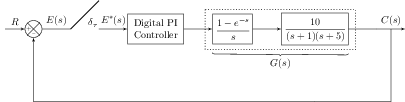
\includegraphics[width=1\linewidth]{Diagrams/block410.pdf}
	\caption*{Figure 4-68}
	\label{fig:samplerblock413}
\end{figure}
Let the PI controller be $\displaystyle G_{PI}(z)=K_p+K_i\frac{1}{1-z^{-1}}=(K_p+K_i)\cfrac{z-\frac{K_p}{K_p-K_i}}{z-1}$ and discretizing $G(s)$
\begin{align*}
& G_{PI}(z)G(z)=G_{PI}(z)\frac{\frac{13711\,z}{100000}+\frac{46027827}{500000000}}{\left(z-\frac{3679}{10000}\right)\,\left(z-\frac{8187}{10000}\right)}=(K_p+K_i)\cfrac{z-\frac{K_p}{K_p-K_i}}{z-1}\frac{0.13711\,z+0.092055654}{\left(z-0.3679\right)\,\left(z-0.8187\right)} \\
& \text{Pick } \frac{\omega_d}{\omega_s}=0.1, \quad \text{since } \zeta=0.5, |z| = \exp \left(\frac{-2\pi \zeta}{\sqrt{1-\zeta^2}}\frac{\omega_d}{\omega_s} \right)=0.6958 \quad \angle z = \frac{360^\circ}{10}= 36^\circ %, z=0.5629 + j0.4090
\end{align*}

% Since the description will be commented out in the final version, could use if package to automatic this process.
\begin{figure}[H]
	\centering
	\includegraphics[width=1\linewidth]{Diagrams/poleszeroes.pdf}
	\caption{Diagram illustrating that the zero $z-\frac{K_p}{K_p-K_i}$ must contribute $125.1015^\circ$}
	\label{fig:polesZeroess}
\end{figure}

\begin{align}
& \notag \angle \left.\left(z-\frac{K_p}{K_p-K_i}\right)\right\vert_{z=0.5629 +j0.4090} = 125.1015^\circ \quad \cfrac{0.409}{0.5629-\frac{K_p}{K_p-K_i}} = \tan(125.1015^\circ) \\
&
\frac{K_p}{K_p-K_i}= 0.850366 \label{eq:kipi1}
\end{align}
\begin{align}
& \notag  (K_p+K_i)\left|\frac{\left(z+0.6714\right)\,\left(0.13711\,z-0.028038995\right)}{(z-0.3679)\,(z-0.8187)}\right|_{z=0.5629 +j0.4090}=1 \\ 
&
0.44357786197\,K_i+0.44357786197\,K_p=1.0 \label{eq:kipi2} 
\end{align}

Solving \eqref{eq:kipi1} and \eqref{eq:kipi2} leads to $K_i=0.33733$ and $K_p=1.9171$.

\[
G_{PI}G(z)=2.254396\cfrac{z-0.850366}{z-1}\frac{0.13711\,(z+0.6714)}{\left(z-0.3679\right)\,\left(z-0.8187\right)}
\]
\begin{align*}
& K_v = \lim\limits_{z \rightarrow 1} \frac{z-1}{z \ T} G_{PI}G(z) = \frac{1}{0.2(1)} \frac{0.149634(0.13711(1.6714))}{(0.6321)(0.1813)}=1.496119
\end{align*}
\subsubsection*{Problem B-4-15}
%Using the Bode diagram approach in the $w$ plane, design a digital controller for the system shown in Figure 4-72. The design specifications are that the phase margin be $50^\circ$, the gain margin be at least 10 dB, and the static velocity error constant $K_v$ be 20 $\text{sec}^{-1}$. The sampling period is assumed to be 0.1 sec, or $T = 0.1$. After the controller is designed, calculate the number of samples per cycle of damped sinusoidal oscillation.

\begin{figure}[H]
	\centering
	\includegraphics[width=1\linewidth]{Diagrams/block415.pdf}
	%\caption*{Figure 4-72}
	\label{fig:samplerblock415}
\end{figure}

\begin{align*}
& G(z) = \mathcal{Z} \left[\frac{1-e^{-sT}}{s}\frac{K}{s(s+0.5)}\right]=0.004918K \frac{z+0.9835}{(z-1)(z-0.9512)}
\end{align*}

Running the \lstinline[language=Matlab]|ass_5.m| in Matlab as with the parameters specified in \textbf{ass\_5.out} results in:
\[
G_DG(z)=\frac{0.32774 z^3 - 0.27218 z^2 - 0.31605 z + 0.26423}{z^4 - 2.7603 z^3 + 2.3775 z^2 - 0.47208 z - 0.14507}
\]
\begin{minipage}[h]{0.5\linewidth}
\begin{figure}[H]
	\centering
	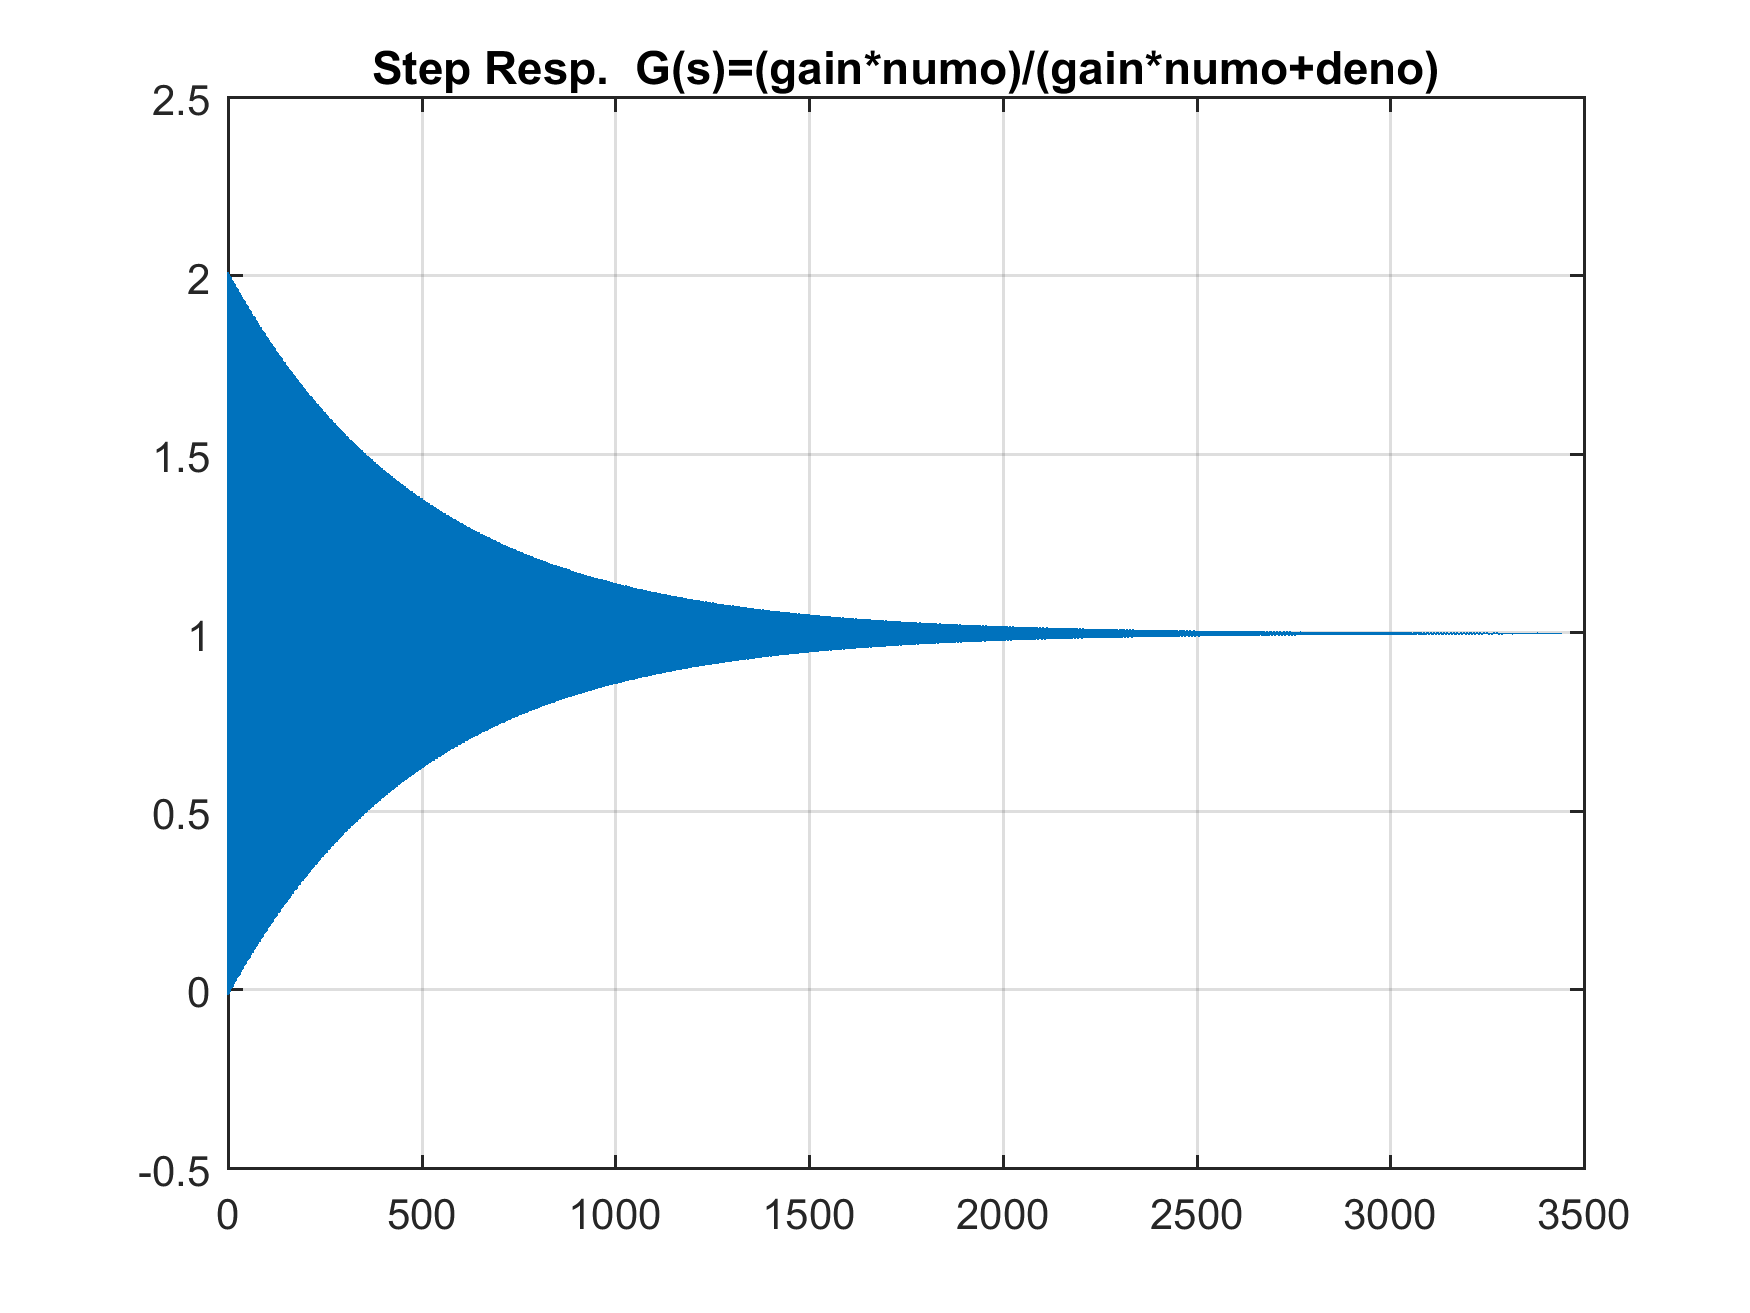
\includegraphics[width=1\linewidth]{MatlabPlots/stepREsp.png}
	\caption{Step Response}
	\label{fig:bodePlotUnComp}
\end{figure}
\end{minipage}
\begin{minipage}[h]{0.5\linewidth}
\begin{figure}[H]
	\centering
	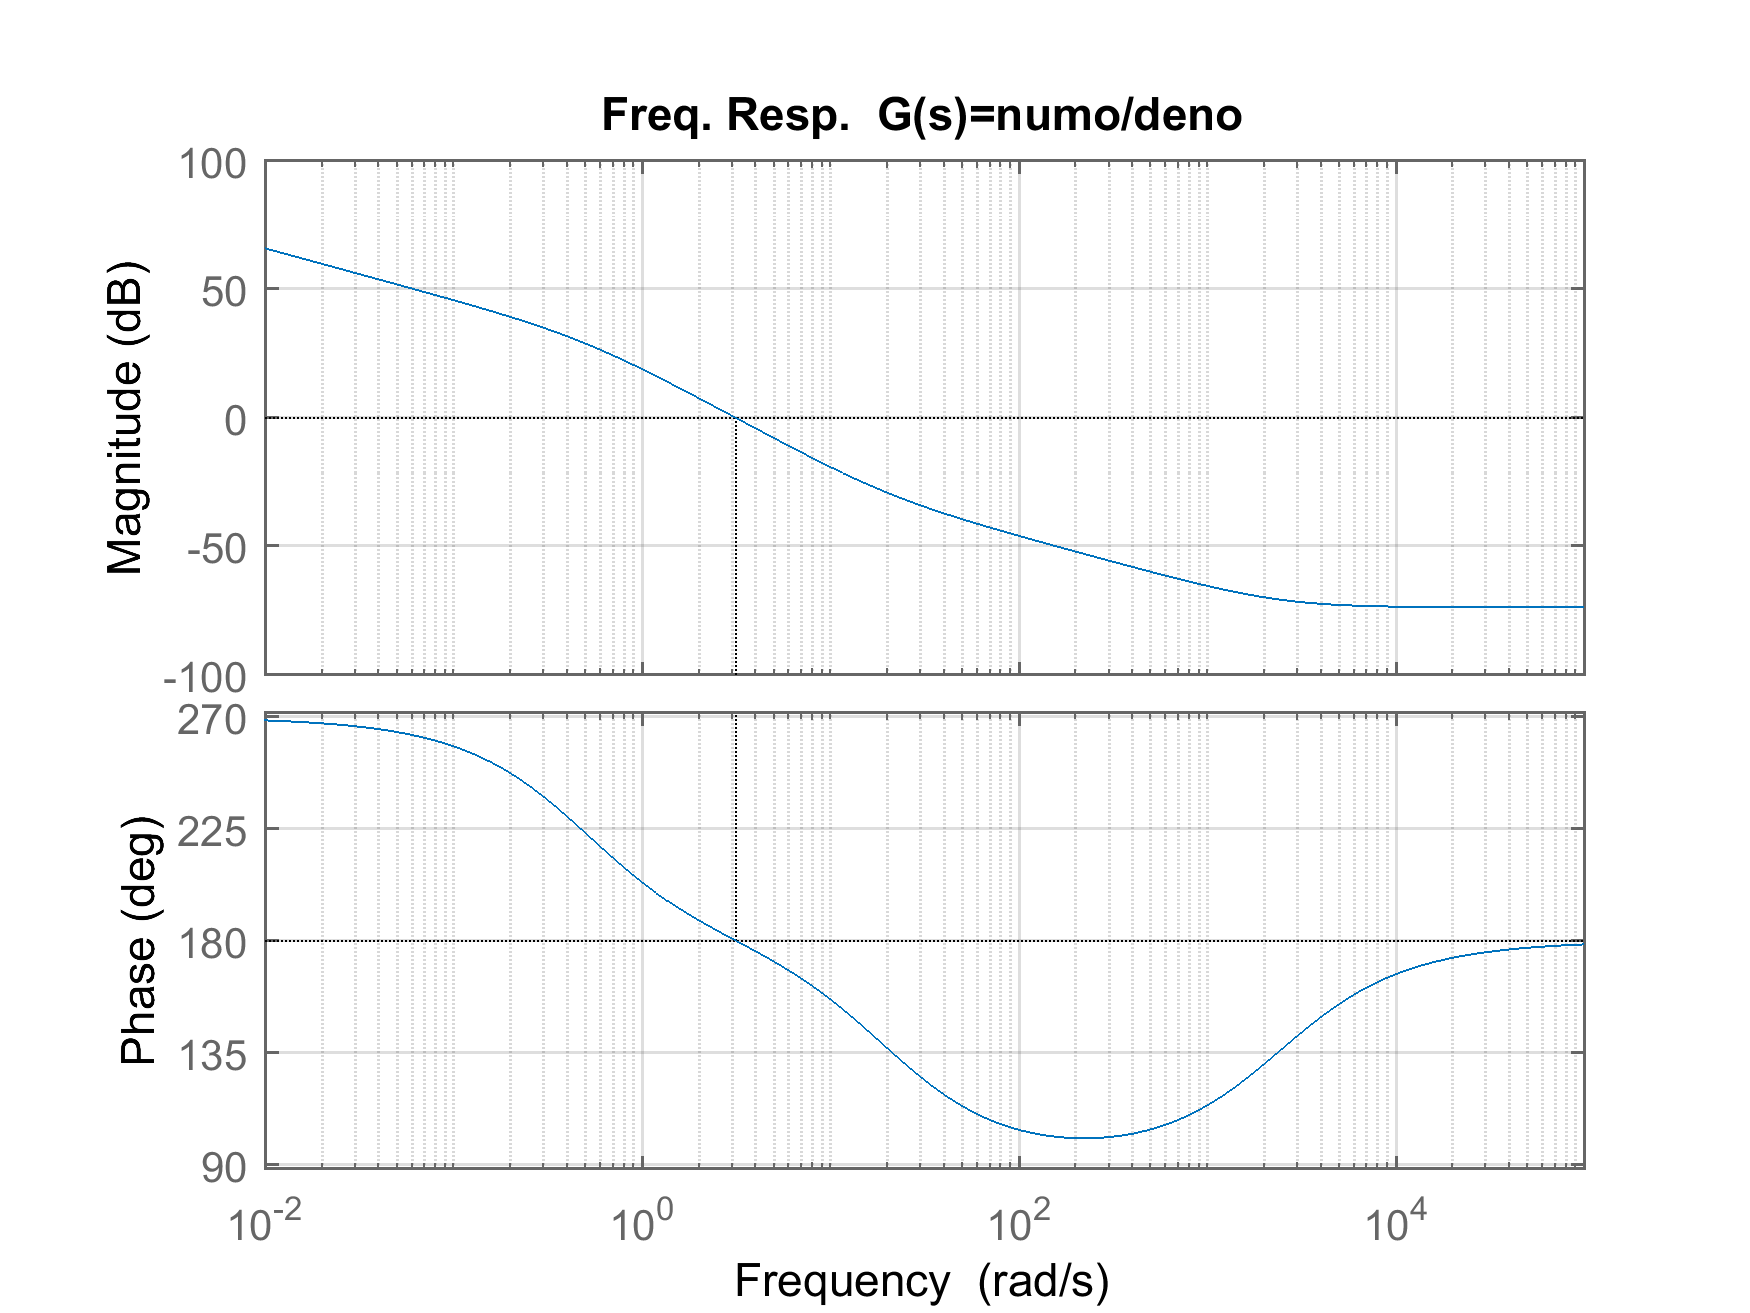
\includegraphics[width=1\linewidth]{MatlabPlots/bodePlotUnComp.png}
	\caption{Bode Plot for uncompensated System}
	\label{fig:bodePlotUnComp}
\end{figure}
\end{minipage}
\begin{figure}[H]
	\centering
	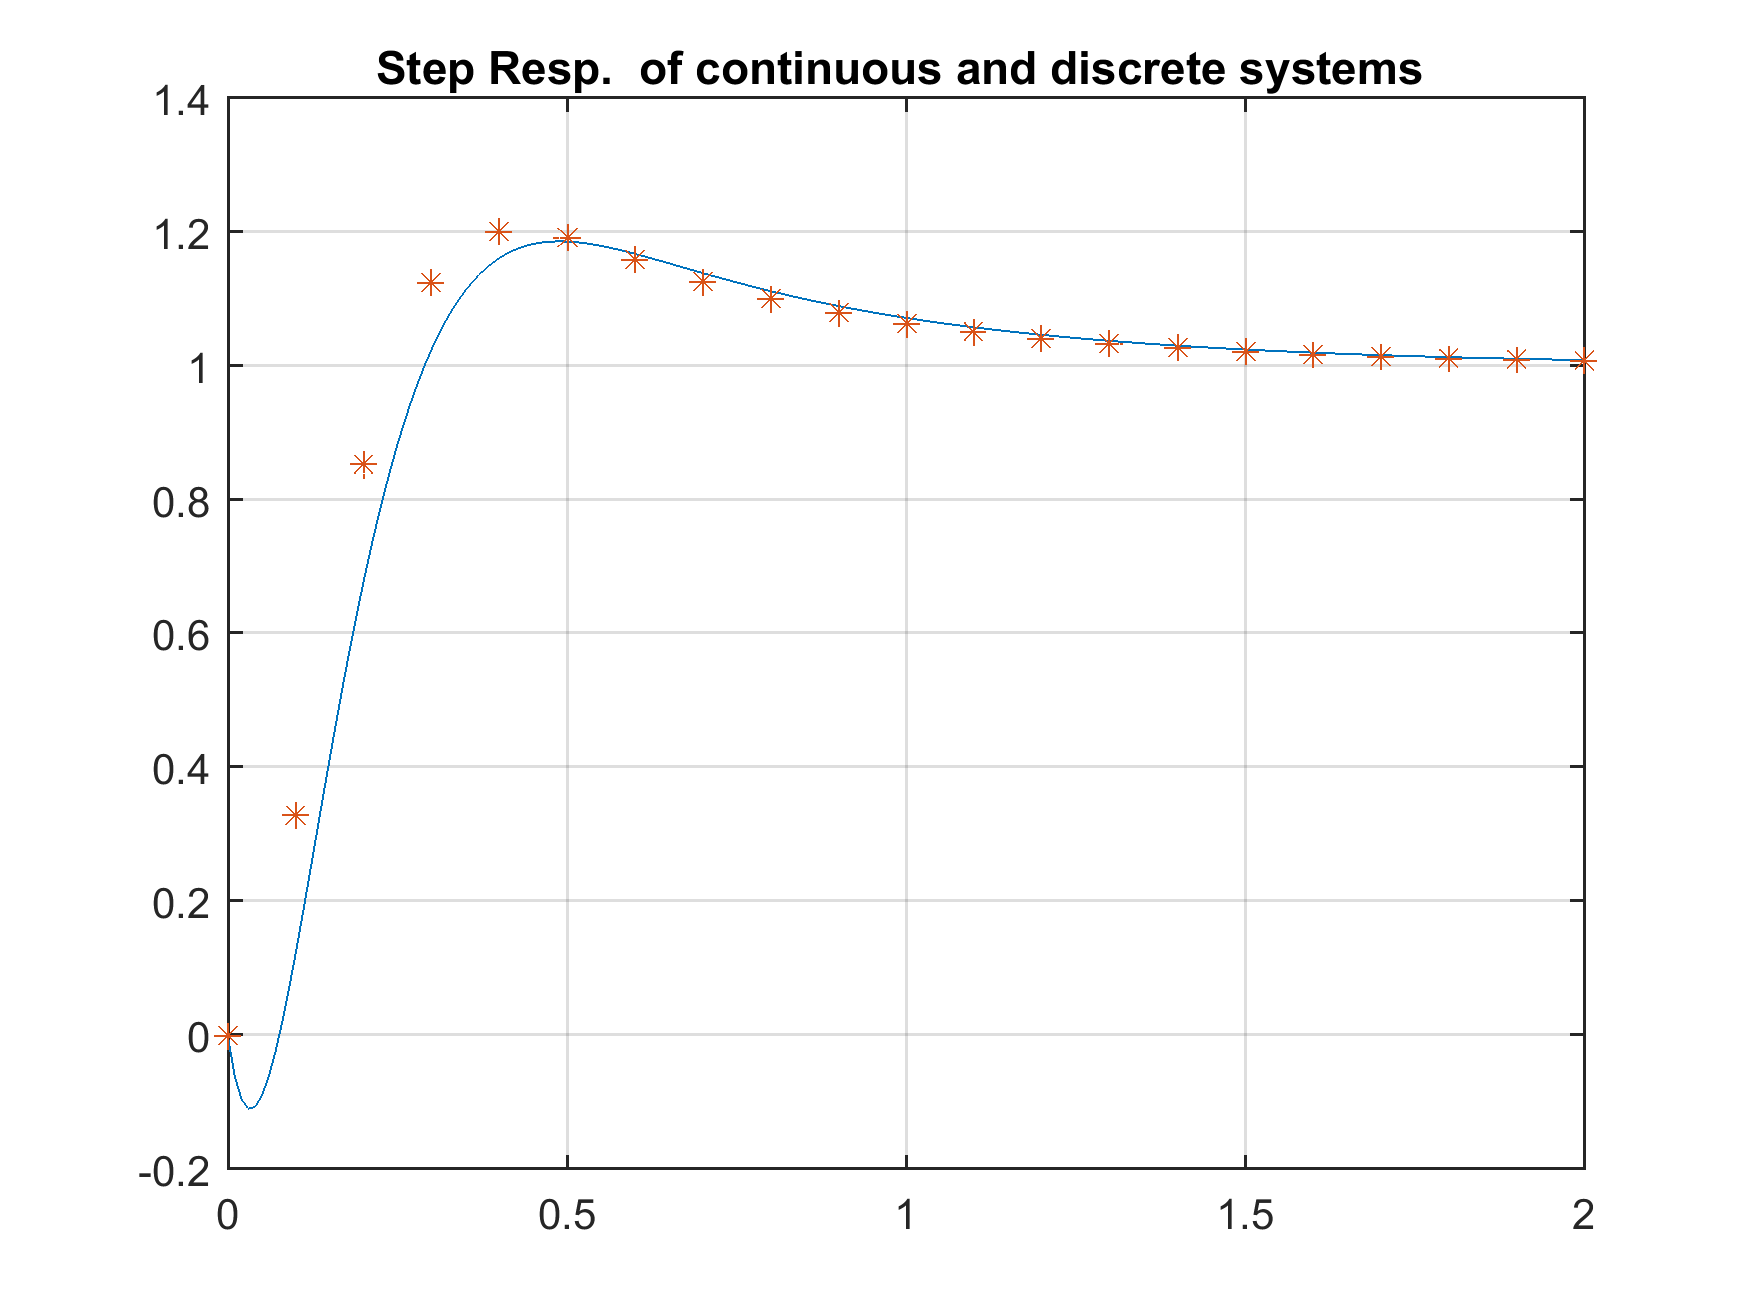
\includegraphics[width=0.6\linewidth]{MatlabPlots/stepRespCTSDS.png}
	\caption{Bode Plot for uncompensated System}
	\label{fig:Step Response}
\end{figure}
\begin{lstlisting}[language=Matlab]
Discrete Compensator): 

num/den = 

66.6418 z^2 - 120.8858 z + 54.6277
----------------------------------
z^2 - 0.80914 z - 0.15251
Open loop compensated discrete system transfer function

num/den = 

0.32774 z^3 - 0.27218 z^2 - 0.31605 z + 0.26423
---------------------------------------------------
z^4 - 2.7603 z^3 + 2.3775 z^2 - 0.47208 z - 0.14507
Closed loop zeros and poles of discrete system
zeros =
	-0.9835
	0.9608
	0.8532
poles =
	0.9607 + 0.0000i
	0.8039 + 0.0000i
	0.3340 + 0.2068i
	0.3340 - 0.2068i
Number of samples per cycle:
ans =
11.3339
\end{lstlisting}

%\begin{lstlisting}[language=Matlab]
%Tts =
%0.1000
%n0d =
%0    0.0049    0.0048
%d0d =
%1.0000   -1.9512    0.9512
%n1 =
%-0.0000   -0.0496    0.9999
%d1 =
%1.0000    0.5002         0
%Enter the vectors of the numerator (numo) and denominator (denum) pol.
%Start with the highest order term. Ex: [1 2 3] corr. (s^2 + 2 s + 3)
%Enter numo: n1
%numo =
%-0.0000   -0.0496    0.9999
%Enter deno: d1
%deno =
%1.0000    0.5002         0
%OPEN-LOOP SYSTEM (without Compensator): 
%
%syso =
%
%-2.079e-05 s^2 - 0.04958 s + 0.9999
%-----------------------------------
%s^2 + 0.5002 s
%
%Continuous-time transfer function.
%
%Enter desired Kv: 20
%Kv =
%20
%Phase margin: 0.075368 at the Gain crossover frq: 3.1629
%Gain margin: 0.072557 in dB at the  Phase crossover frq:3.1765
%Zeros and poles of closed-loop system without compensator:
%zeros =
%1.0e+03 *
%-2.4042
%0.0200
%poles =
%-0.0021 + 3.1633i
%-0.0021 - 3.1633i
%Damping: 0.00065785, Overshoot: 0.99794, Settling time: 1922.2057
%Press CR to continue
%Press CR to continue
%Phase lead in degrees: 63
%a =
%0.0576
%Kc =
%173.5888
%Warning: The closed-loop system is unstable. 
%> In ctrlMsgUtils.warning (line 25)
%In DynamicSystem/margin (line 65)
%In margin (line 100)
%In lead_c (line 122)
%In ass_5 (line 30) 
%At wc= 6.6156 the gain of the transfer function is equal to sqrt(a).
%Use this frequency as the new gain crossover frequency wc
%Enter wc, the new gain crossover frequency : 6.6
%Compensator: 
%
%num/den = 
%
%s + 1.5845
%----------
%s + 27.491
%Compensator gain: 173.5888
%Compensated Open-Loop trsf. function;
%
%num/den = 
%
%-0.0036096 s^3 - 8.6119 s^2 + 159.9316 s + 275.0225
%---------------------------------------------------
%s^3 + 27.9912 s^2 + 13.7511 s
%Phase margin: 49.1318 at the Gain crossover frq: 6.6301
%Gain margin: 9.7093 in dB at the  Phase crossover frq:22.5492
%Zeros and poles of Closed-loop system with compensator:
%zeros =
%1.0e+03 *
%-2.4042
%0.0200
%-0.0016
%poles =
%-8.7376 + 7.9666i
%-8.7376 - 7.9666i
%-1.9742 + 0.0000i
%Closed loop system has a real dominant pole
%Press CR to continue
%Press CR to continue
%Enter >0 to continue) :0
%decision =
%0
%n2 =
%-0.0036   -8.6119  159.9316  275.0225
%d2 =
%1.0000   27.9912   13.7511         0
%Enter the vectors of the numerator (numo) and denominator (denum) pol.
%Start with the highest order term. Ex: [1 2 3] corr. (s^2 + 2 s + 3)
%Both vectors should have the same length
%Enter numo: n2
%numo =
%-0.0036   -8.6119  159.9316  275.0225
%Enter deno: d2
%deno =
%1.0000   27.9912   13.7511         0
%OPEN-LOOP SYSTEM (without Compensator): 
%
%num/den = 
%
%-0.0036096 s^3 - 8.6119 s^2 + 159.9316 s + 275.0225
%---------------------------------------------------
%s^3 + 27.9912 s^2 + 13.7511 s
%Enter desired Kv: 20
%Kv =
%20
%Phase margin "Pm" at the Gain crossover frq. "Wcp" 
%Pm =
%49.1318
%Wcp =
%6.6301
%Gain margin "Gm" in dB at the  Phase crossover frq " Wcg" 
%Gm =
%9.7093
%Wcg =
%22.5492
%Zeros and poles of closed-loop system without compensator:
%zeros =
%1.0e+03 *
%-2.4042
%0.0200
%-0.0016
%poles =
%-8.7376 + 7.9666i
%-8.7376 - 7.9666i
%-1.9742 + 0.0000i
%Settling time "sett" and zeta "zeta" of same closed-loop system:
%sett =
%0.4578
%zeta =
%0.7390
%Press CR to continue
%Press CR to continue
%Desired Phase margin in degrees (include an allowance for the effect of lag compensator): 52
%Phase margin is "degree" degrees at w = "Wcg".
%degree =
%52
%Wcg =
%5.6755
%Try another Phase margin? (y/n): n
%Enter wc, new gain crossover frequency: 5.6
%wc =
%5.6000
%Location of the zero of the compensator: 0.4
%beta =
%1.1876
%bTt =
%0.3368
%Kc =
%0.8421
%Compensator: 
%
%num/den = 
%
%s + 0.4
%-----------
%s + 0.33683
%Compensator gain Kc: 
%Kc =
%0.8421
%Compensated Open-Loop trsf. function;
%
%num/den = 
%
%-0.0030395 s^4 - 7.2531 s^3 + 131.7724 s^2 + 285.4567 s + 92.635
%----------------------------------------------------------------
%s^4 + 28.328 s^3 + 23.1793 s^2 + 4.6317 s
%Phase margin "Pm" at the Gain crossover frq. "Wcp" 
%Pm =
%51.6267
%Wcp =
%5.6046
%Gain margin "Gm" in dB at the  Phase crossover frq " Wcg" 
%Gm =
%11.1797
%Wcg =
%22.4811
%Zeros and poles of Closed-loop system with compensator:
%zeros =
%1.0e+03 *
%-2.4042
%0.0200
%-0.0016
%-0.0004
%poles =
%-9.2826 + 4.5388i
%-9.2826 - 4.5388i
%-2.1736 + 0.0000i
%-0.4004 + 0.0000i
%Settling time "sett" and zeta "zeta" of compens. closed-loop system:
%sett =
%0.4309
%zeta =
%0.8984
%Press CR to continue
%Press CR to continue
%Enter decision ( >0 to continue) :0
%decision =
%0
%n3 =
%-0.0030   -7.2531  131.7724  285.4567   92.6350
%d3 =
%1.0000   28.3280   23.1793    4.6317         0
%Discrete Compensator): 
%
%num/den = 
%
%66.6418 z^2 - 120.8858 z + 54.6277
%----------------------------------
%z^2 - 0.80914 z - 0.15251
%Open loop compensated discrete system transfer function
%
%num/den = 
%
%0.32774 z^3 - 0.27218 z^2 - 0.31605 z + 0.26423
%---------------------------------------------------
%z^4 - 2.7603 z^3 + 2.3775 z^2 - 0.47208 z - 0.14507
%Closed loop zeros and poles of discrete system
%zeros =
%-0.9835
%0.9608
%0.8532
%poles =
%0.9607 + 0.0000i
%0.8039 + 0.0000i
%0.3340 + 0.2068i
%0.3340 - 0.2068i
%Number of samples per cycle:
%ans =
%11.3339
%\end{lstlisting}

%\subsubsection*{Problem B-3-20}
%Assuming that the sampling period is 0.2 sec, and the gain constant K is unity, determine the response c(kT) for k = 0,1,2,3 and 4 when the input r(t) is a unit-step function. Also, determine the final value $c(\infty)$.
%\begin{figure}[H]
%	\centering
%	\includegraphics[width=0.6\linewidth]{Diagrams/samplerBlock.pdf}
%	\caption{Block Diagram for B-3-20}
%	\label{fig:samplerblock}
%\end{figure}
%
%Table 3-1 from the textbook %\cite{ogataDiscrete}
% $C(z)=\frac{[GR(z)]}{1+GH(z)}$, where $GH(z) = \left[G(s)H(s)\right]^\ast=[1-z^{-1}] \mathcal{Z} \left\{\frac{1}{s(s+1)}\right\}$
%\begin{align*}
%&  \mathcal{Z} \left\{\frac{1}{s(s+1)}\right\} = \mathcal{Z} \left\{\frac{1}{s}+\frac{-1}{s+1}\right\} = \frac{z}{z-1}-\frac{z}{z-e^{-(0.2)(1)}}=\frac{z}{(z-1)(z-e^{-0.2})} \\
%& GH(z) = \left[G(s)H(s)\right]^\ast=[1-z^{-1}] \mathcal{Z} \left\{\frac{1}{s(s+1)}\right\} 
%= 1-\frac{z-1}{z-e^{-0.2}}=\frac{1-e^{-0.2}}{z-e^{-0.2}}=\frac{0.181269}{z-0.818731} \\
%& R(z)G(z)= \mathcal{Z} \left\{\frac{1}{s}\frac{1}{(s+1)}\right\} = \frac{0.181269z}{(z-1)(z-0.818731)} \\
%& C(z) =\cfrac{\frac{0.181269z}{(z-1)(z-0.818731)}}{1+\frac{0.181269}{z-0.818731}}= \cfrac{\frac{0.181269z}{(z-1)(z-0.818731)}}{\frac{z-0.818731+0.181269}{z-0.818731}}= \cfrac{0.1813z}{(z-1)(z-0.8187)} \times \cfrac{z-0.819}{z-0.637}=\cfrac{0.1813z}{(z-1)(z-0.6375)} 
% %\frac{z^2}{(z-1)(z-0.818731)}
%\end{align*}
%Using final value theorem:
%
%\[ c(\infty)=\lim\limits_{z\rightarrow 1} \left[ \left(1-z^{-1}\right)C(z)\right]=\lim\limits_{z\rightarrow 1} \left[ \left(1-z^{-1}\right)\cfrac{0.1813z^{-1}}{(1-z^{-1})(1-0.6375z^{-1})} \right]=0.5001379 \]
%\subsubsection*{Problem B-4-4}
%Consider the discrete-time closed-loop control system shown in Figure 4-13. Determine
%the range of K for stability by use of the Jury stability criterion. Assuming that $T=1$.
%
%\begin{figure}[H]
%	\centering
%	\includegraphics[width=1\linewidth]{Diagrams/sampler413.pdf}
%	\caption*{Figure 4-13}
%	\label{fig:samplerblock413}
%\end{figure}
%
%\begin{align*}
%&(1-z^{-1}) \mathcal{Z} \left\{ \frac{1}{s^2}\frac{1}{s+1} \right\}= (1-z^{-1}) \mathcal{Z} \left\{ \frac{1}{s^2}+\frac{-1}{s}+\frac{1}{s+1} \right\} =  \left(\frac{Tz^{-1}}{1-z^{-1}}-1+\frac{1-z^{-1}}{1-e^{-1}z^{-1}}\right) \\
%& = \frac{z^{-1}}{1-z^{-1}}-1+\frac{1-z^{-1}}{1-e^{-1}z^{-1}} =\frac{z^{-1}-e^{-1}z^{-2}
%	-(1-e^{-1}z^{-1}+e^{-1}z^{-2}) +(1-2z^{-1}+z^{-2}
%	)}{(1-z^{-1})(1-e^{-1}z^{-1})} \\
%& = \frac{e^{-1}z^{-1}+(1-2e^{-1})z^{-2}}{(1-z^{-1})(1-e^{-1}z^{-1})} \quad G(z) = \frac{K[e^{-1}z^{1}+(1-2e^{-1})]}{(z-1)(z-e^{-1})} \quad \frac{C(s)}{R(s)}=\frac{G(z)}{1+G(z)(1)} \\
%& P(z)= a_0z^2+a_1z+a_2=z^2-(1.3679-0.3679K)z+(0.3679+0.2642K) \\
%& |a_2| < |a_0| \quad |0.3679+0.2642K| < |1| \rightarrow K =2.3925056 \\
%& P(1) > 0 \ 1-1.3679-0.3679K + 0.3679+0.2642K > 0 \rightarrow 0.6321K > 0 \\
%& P(-1) > 0 \ 1+(1.3679-0.3679K)+0.3679+0.2642K > 0 \quad 2.7358-0.1037K > 0 \ K > 26.3818
%\end{align*}
%For stability $0 < K < 2.3925056$.
%
%\subsubsection*{Problem B-4-8}
%Consider the digital control system shown in Figure 4-66. Plot the root loci as the gain K is varied from $0$ to $\infty$. Determine the critical value of gain K for stability. The sampling period is 0.1 sec, or $T=0.1$ What value of gain K will yield a damping ration $\zeta$ of the closed-loop poles equal to 0.5? With gain K set to yield $\zeta=0.5$, determine the damped natural frequency $\omega_d$ and the number of samples per cycle of damped sinusoidal oscillation.
%
%\begin{minipage}[h]{0.5\linewidth}
%\begin{figure}[H]
%	\centering
%	\includegraphics[width=1\linewidth]{Diagrams/B4-8.pdf}
%	\caption*{Figure 4-66 with $T=0.1$}
%	\label{fig:samplerblock48}
%\end{figure}
%\vspace*{-1.05cm}
%\begin{align*}
%P(z)&=(z-1)(z-0.6065)+K(z+1) \\
%    s&=z^2+(K-1.6065)z+(0.6065-K) \\
%    & |a_2| < |a_0| \rightarrow |0.6065+K| < 1 \quad K =0.3935 \\
%    & P(1) > 0 \rightarrow 2K > 0 \\
%    & P(-1) > 0 \rightarrow 3.213 > 0 \\
%    & 0 < K < 0.3935
%\end{align*}
%\end{minipage}
%\begin{minipage}[h]{0.5\linewidth}
%\begin{figure}[H]
%	\centering
%	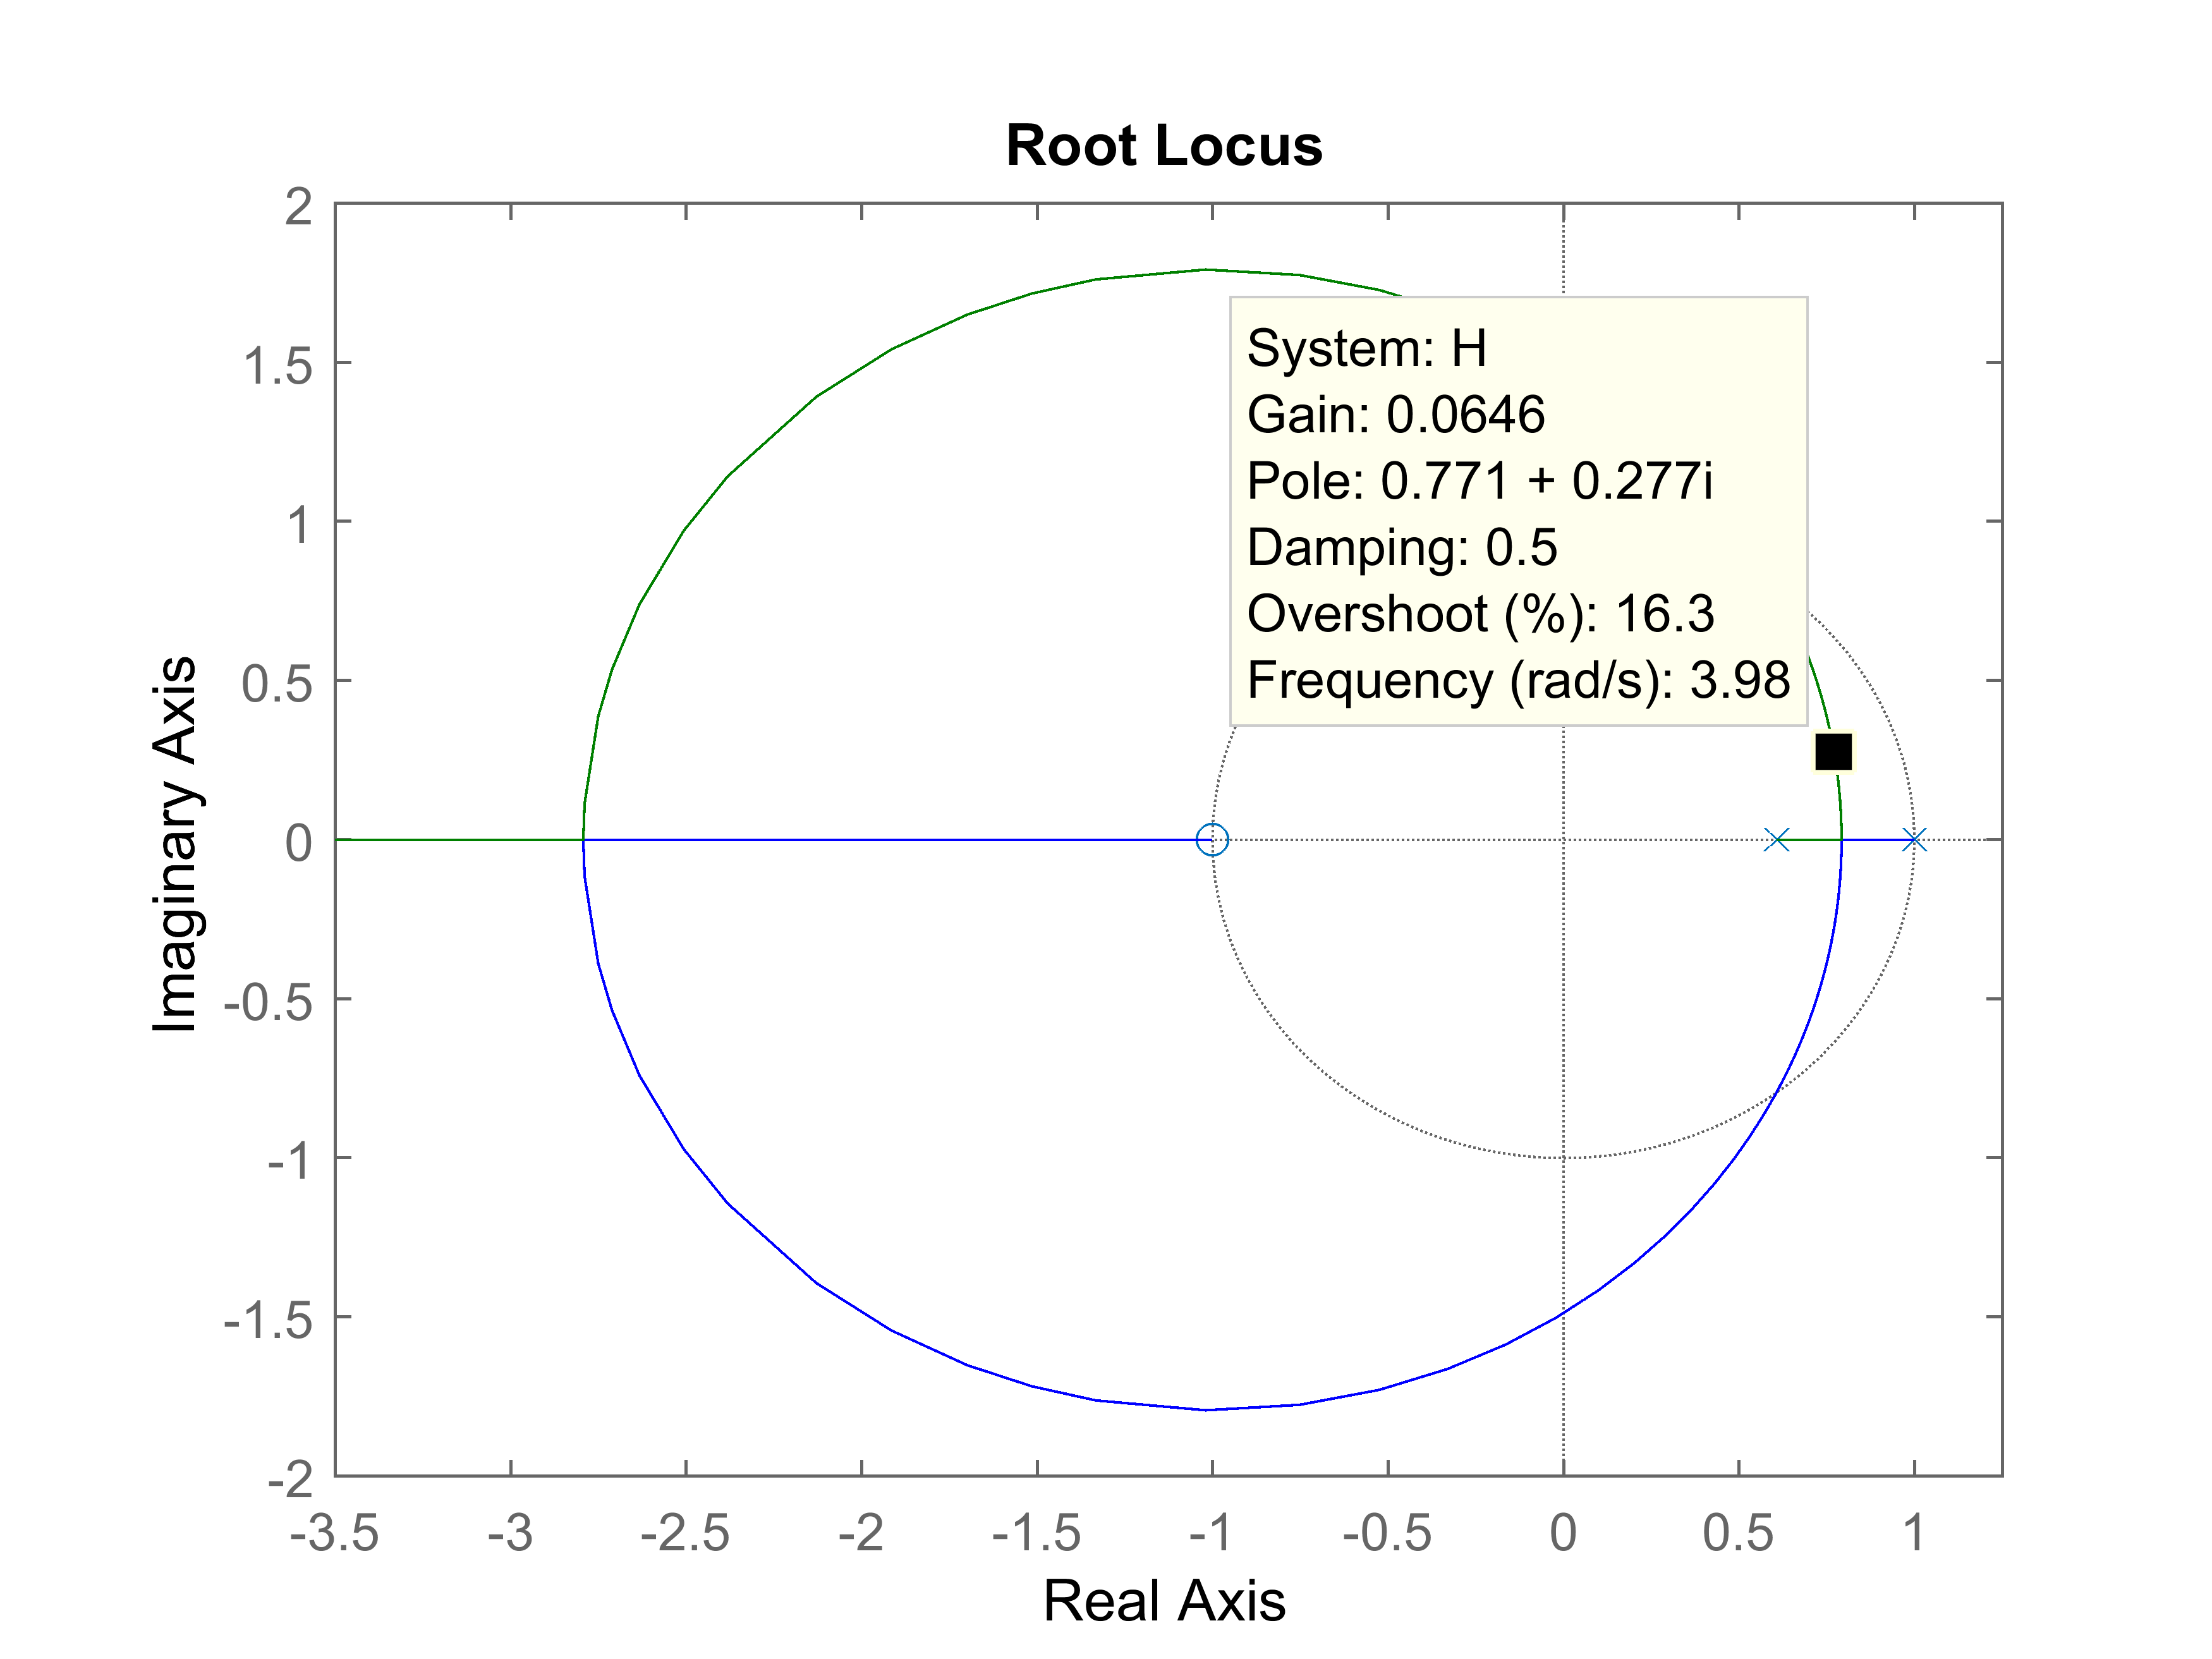
\includegraphics[width=1\linewidth]{Diagrams/B-4-8Rlocus2.png}
%	\caption*{Root Locus For Figure 4-66}
%	\label{fig:Rlocus}
%\end{figure}
%\end{minipage}
%When $K=0.0646, \zeta=0.5$ with the pole at $z=0.771+j0.277=|0.8192|e^{j19.7620^\circ}$. 
%\begin{align*}
%z=  & |e^{-T(\zeta \omega_n)} |e^{T \omega_d} = |0.8192|e^{j19.7620^\circ} \\
%& \omega_n = \frac{\ln(0.8192)}{(-0.1)(0.5)}=3.98854 = 4 \ \text{rad/s} \\
%& \omega_d = \frac{(19.7629^\circ)}{0.1} = 3.449 \quad  \omega_d = \omega_n \sqrt{1-\zeta^2}=3.988 (0.866025)=3.4537 \ \text{rad/s} \\
%& \text{Number of Samples per Cycle } = \frac{360^\circ}{T\omega_d}=\frac{360^\circ}{19.7629^\circ}=18.22
%\end{align*}
%	 %$P(z)=z^2-1.5419z+0.5419$, %$2 \zeta \omega_n =-1.5419$
%%\begin{figure}[H]
%%	\centering
%%	\includegraphics[width=1\linewidth]{Diagrams/B4-8.pdf}
%%	\caption*{Figure 4-66}
%%	\label{fig:samplerblock48}
%%\end{figure}
%
%
%\subsubsection*{Problem B-4-12}
%Design a digital proportional-plus-derivative controller for the plant whose transfer function is $1/s^2$, as shown in Figure 4-70. It is desired that the damping ratio $\zeta$ of the dominant closed-loop poles be 0.5 and the undamped natural frequency be 4 rad/sec. The sampling period is 0.1 sec, or $T=0.1$. After the controller is designed, determine the number of samples per cycle of damped sinusoidal oscillation.
%\begin{figure}[H]
%	\centering
%	\includegraphics[width=1\linewidth]{Diagrams/block412.pdf}
%	\caption*{Figure 4-70}
%	\label{fig:blockB4-12}
%\end{figure}
%% https://www.wolframalpha.com/input/?i=inverse+laplace+transform+of+s
%\vspace*{-1.05cm}
%\begin{align*}
%&  G_{PD}(s) = K_ds +K_p \quad G(z) = (1-z^{-1}) \mathcal{Z} \left\{\frac{1}{s^3} \right\} = \frac{(1-z^{-1})}{2} \mathcal{Z} \left\{\frac{2}{s^3} \right\} = \frac{(1-z^{-1})}{2} \frac{T^2z^{-1}(1+z^{-1})}{(1-z^{-1})^3} \\
%& G_{PD}(z) =K_p+K_d(1-z^{-1})= (K_p+K_d)\cfrac{z-\frac{K_d}{K_p+K_d}}{z}, \quad G(z)=\frac{T^2z^{-1}(1+z^{-1})}{2(1-z^{-1})^2}=0.005\frac{(z+1)}{(z-1)^2} \\
%& \omega_d = \omega_n \sqrt{1-\zeta^2} = 4 \sqrt{1-0.5^2}= 2 \sqrt{3} =3.4641 \ \text{rad/s}, \quad |z| = e^{T \zeta \omega_n} = e^{-T \zeta \omega_n} =e^{-0.2} = 0.8187 \\
%& \angle z = \angle T \omega_d = 0.34641 \ \text{rad} =19.8478^\circ \quad  \text{Desired Pole } z = 0.8187 \angle 19.8478^\circ =0.7701+j0.2780 \\
%& G_{PD}(z)G(z)= (K_p+K_d)\cfrac{z-\frac{K_d}{K_p+K_d}}{z}0.005\frac{(z+1)}{(z-1)^2}
%\end{align*}
%
%Computing the angle deficiency:
%% https://www.wolframalpha.com/input/?i=1%2F(-0.2299%2Bi*0.2780)%5E2
%% https://www.wolframalpha.com/input/?i=atan(0.2780%2F(0.7701-x))%2Bpi%3D0.500055555*pi
%\begin{align*}
%& % \left. \phase{\frac{1}{(z-1)^2}}\right \vert_{z=0.7701+j0.2780}
%\phi_1=\phase{\frac{1}{(z-1)^2}} \bigg\vert_{z=0.7701+j0.2780} = \phase{\frac{1}{(-0.2299+j0.2780)^2}}= 100.82^\circ \quad \phi_2=\phase{z+1}\vert_{z=0.7701+j0.2780} =8.9255^\circ \\
%& \phi_3 = \phase{\frac{1}{z}} \bigg\vert_{z=0.7701+j0.2780} =-19.84918^\circ \quad  \phi=180^\circ-\phi_1 -\phi_2-\phi_3=90.10^\circ \\
%&\phi = \phase{z-\frac{K_d}{K_p+K_d}}\bigg\vert_{z=0.7701+j0.2780}=90.10^\circ \rightarrow \tan^{-1} \left({\cfrac{0.2780}{0.7701-\frac{K_d}{K_p+K_d}}} \right) + 180^\circ= 90.10^\circ \\
%& \frac{K_d}{K_p+K_d} = 0.770149 \rightarrow G_{PD}(z)G(z)= (K_p+K_d)\cfrac{z-0.770149 }{z}0.005\frac{(z+1)}{(z-1)^2}
%\end{align*}
%\begin{align}
%& \frac{K_d}{K_p+K_d} = 0.770149 \\
%&\left|(K_p+K_d)\cfrac{z-0.770149 }{z}0.005\frac{(z+1)}{(z-1)^2} \right|\bigg\vert_{z=0.7701+j0.2780} =1
%\end{align}
%Solving for equations (1) and (2),
%
%\[ 
%K_p=9.833174968 \quad  K_d=32.9474741
%\]
%
%The controller $\displaystyle G_{PD}=42.7806\frac{z-0.770149}{z} = 42.7806(1-0.770149z^{-1})$. The number of cycles per second $n=\frac{360^\circ}{19.84918^\circ}=18.13678$
\end{document}

    
